% ===================== RESUMEN EJECUTIVO =====================
\newpage
\section*{Resumen Ejecutivo}
\addcontentsline{toc}{section}{Resumen Ejecutivo}

El presente estudio técnico, encomendado por \textbf{Ingredion S.A.} a \textbf{DML Ingenieros Consultores S.A.S.}, proporciona un análisis integral de transferencia de calor e integridad estructural del tanque de almacenamiento de glucosa Globe 1130 (223 m$^3$) en la planta de Cali, Colombia. La investigación se centra en la optimización del sistema de calentamiento por media caña en espiral y la validación de la seguridad operativa bajo condiciones críticas de carga hidrostática y térmica, empleando un enfoque metodológico que combina cálculos analíticos con simulación numérica avanzada (CFD y FEA).

\subsection*{Escenarios de Operación Evaluados}

Se definieron cuatro escenarios base para caracterizar la respuesta térmica del sistema frente a variaciones en el volumen de llenado y la temperatura del fluido de servicio (agua caliente), tal como se detalla en la Tabla~\ref{tab:resumen_escenarios}.

\begin{table}[H]
	\centering
	\caption{Descripción de los escenarios de simulación térmica.}
	\label{tab:resumen_escenarios}
	\setcounter{itemcount}{0}
	\begin{tabularx}{\textwidth}{@{}lXcc@{}}
		\toprule
		\textbf{Escenario} & \textbf{Descripción Operativa} & \textbf{Llenado [\%]} & \textbf{T$_{agua}$ [°C]} \\
		\midrule
		Escenario 1 & Calentamiento de volumen parcial (lote inicial) & 7.6\% (24 m$^3$) & 65 \\
		Escenario 2 & Operación estándar de inventario masivo & 80.0\% (178 m$^3$) & 65 \\
		Escenario 3 & Optimización térmica (incremento de gradiente) & 80.0\% (178 m$^3$) & 75 \\
		Escenario 4 & Ciclo industrial de despacho (8 carrotanques) & Variable & 75 \\
		\bottomrule
	\end{tabularx}
\end{table}

\subsection*{Análisis de Resultados Técnicos}

Los indicadores clave de desempeño (KPI) derivados del análisis transitorio revelan una dependencia crítica de la viscosidad del jarabe ($>212,000$ cP a 20°C). El incremento de la temperatura del agua de 65°C a 75°C (Escenario 3) genera una \textbf{reducción del 46\%} en el tiempo de preparación logística para alcanzar los 57°C operativos, pasando de 772.8 a 415.2 horas (ver Tabla~\ref{tab:resumen_kpi}).

\begin{table}[H]
	\centering
	\caption{Comparativa de indicadores de desempeño térmico y estructural.}
	\label{tab:resumen_kpi}
	\setcounter{itemcount}{0}
	\begin{tabularx}{\textwidth}{@{}Xccc@{}}
		\toprule
		\textbf{Parámetro de Control} & \textbf{Escenario 2} & \textbf{Escenario 3} & \textbf{Límite / Meta} \\
		\midrule
		Coeficiente Global $U$ [W/m$^2\cdot$°C] & 17.9 -- 28.0 & 21.1 -- 36.2 & Maximizar \\
		Tiempo a 57°C (80\% llenado) & 772.8 h & 415.2 h & Minimizar \\
		Eficiencia de Aislamiento (2'') & 91.0\% & 91.0\% & $>90\%$ \\
		Factor de Seguridad (FS) @ 90\% & 1.05 & 1.05 & $>1.0$ (ASME) \\
		Factor de Seguridad (FS) @ 100\% & 0.71 & 0.71 & \textbf{Crítico} \\
		\bottomrule
	\end{tabularx}
\end{table}

El análisis de resistencias térmicas demuestra que la \textbf{convección natural de la glucosa concentra el 98.0\% de la resistencia total} del sistema. La validación mediante \textbf{CFD (COMSOL Multiphysics)} confirmó un coeficiente $U$ de 38 W/m$^2\cdot$°C en estado estable, validando la precisión del modelo analítico con una desviación del 5\%. La Figura~\ref{fig:resumen_cfd} ilustra el enfriamiento del agua en la espiral y la alta inercia térmica del producto.

\begin{figure}[H]
	\centering
	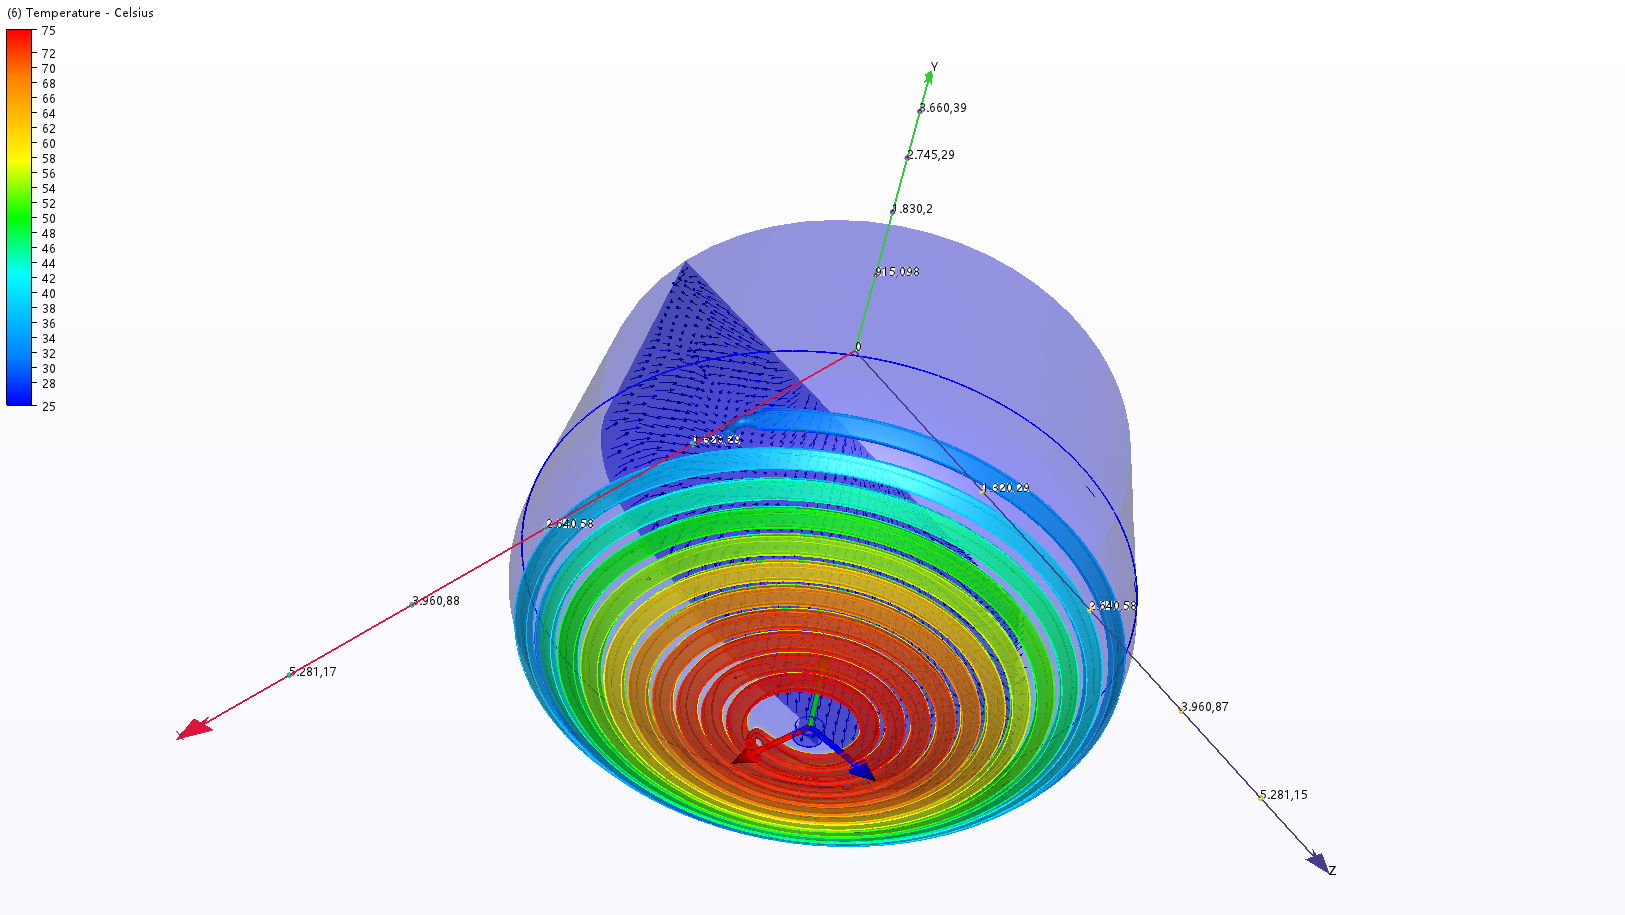
\includegraphics[width=0.75\textwidth]{../figures/cfd1.png}
	\caption{Simulación CFD: Perfiles de temperatura en el fondo toriesférico y chaqueta espiral. Se observa la dominancia de la resistencia térmica del lado del producto durante el arranque.}
	\label{fig:resumen_cfd}
\end{figure}

\subsection*{Capacidad Volumétrica y Límites de Seguridad}

Se define la \textbf{Capacidad Nominal (100\%)} como el volumen total del cuerpo cilíndrico más el fondo toriesférico (\textbf{222.8 m$^3$}), excluyendo explícitamente el volumen del techo superior, el cual debe reservarse como espacio de vapor (\textit{ullage}). 

Bajo esta definición, el análisis de integridad estructural determina que el \textbf{Volumen Máximo Operativo de Seguridad es de 200.5 m$^3$ (90\% de la capacidad nominal)}. Operar por encima de este umbral reduce el Factor de Seguridad (FS) por debajo de la unidad en la unión fondo-cilindro, incrementando el riesgo de deformación plástica y fatiga prematura del activo.

\begin{figure}[H]
	\centering
	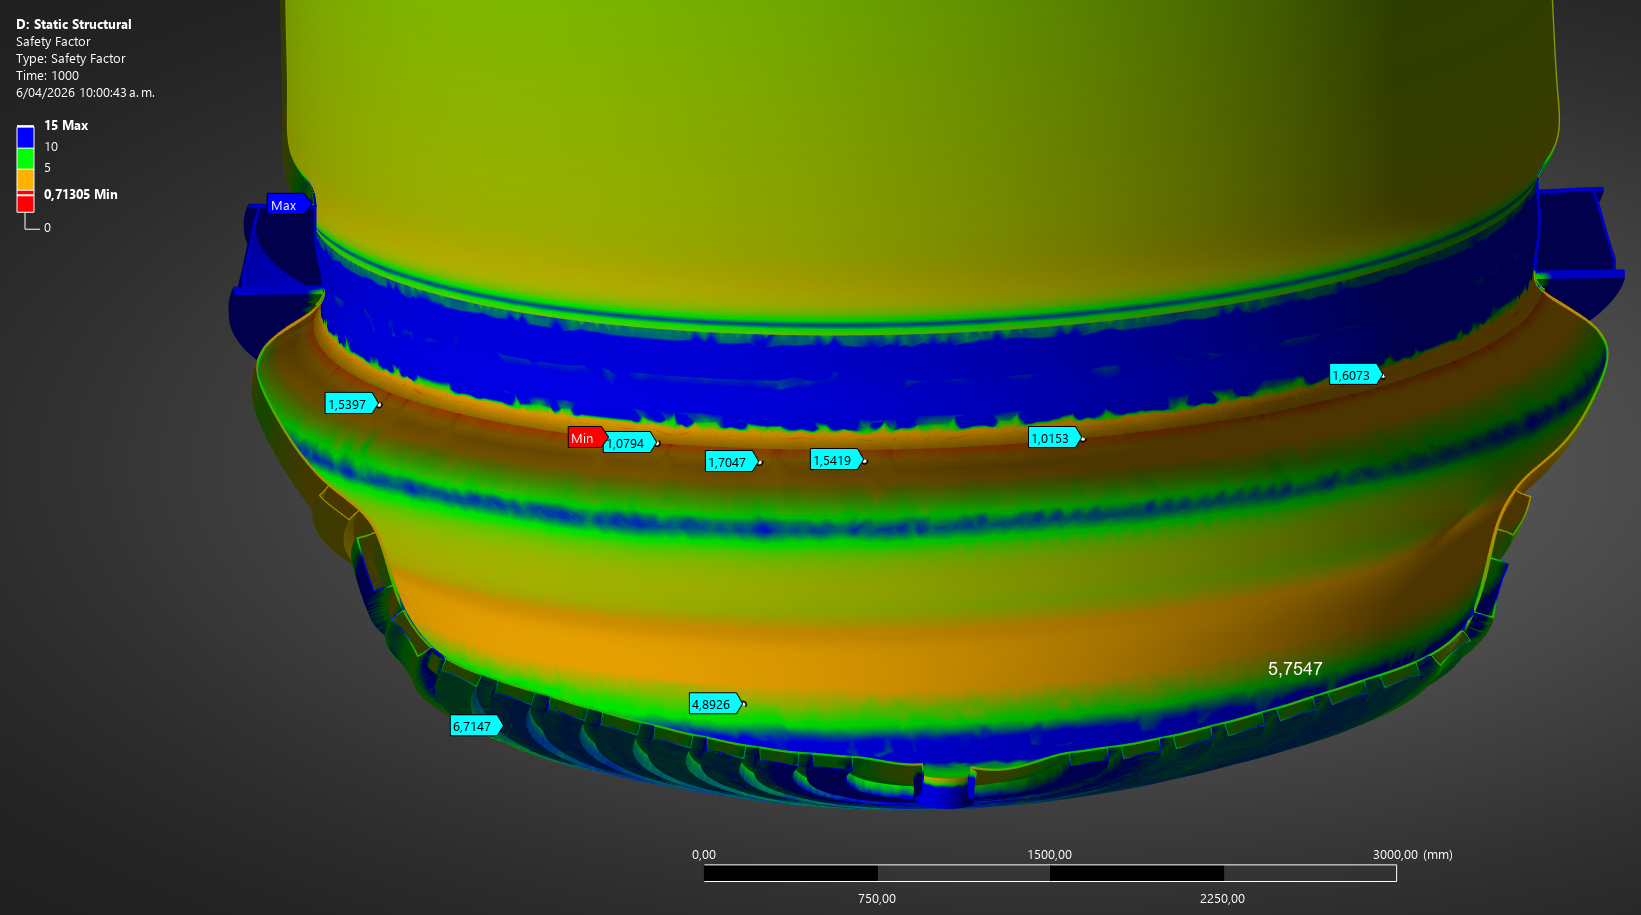
\includegraphics[width=0.75\textwidth]{../figures/fea3.png}
	\caption{Distribución del Factor de Seguridad (FEA). Las zonas en rojo ($FS < 1.0$) localizadas en el nudillo y anclajes de chaqueta indican la necesidad de control de nivel estricto.}
	\label{fig:resumen_fea}
\end{figure}

\subsection*{Dinámica del Ciclo de Despacho}

El \textbf{Escenario 4} modela la logística de despacho de 192 toneladas. El análisis concluye que, tras un recalentamiento inicial de \textbf{25.5 horas} (de 55°C a 57°C), es posible ejecutar las 8 cargas de forma consecutiva sin interrupciones por temperatura, manteniendo el producto entre 57°C y 60°C. El ciclo completo requiere un tiempo de ventana de \textbf{37.5 horas}.

\begin{figure}[H]
	\centering
	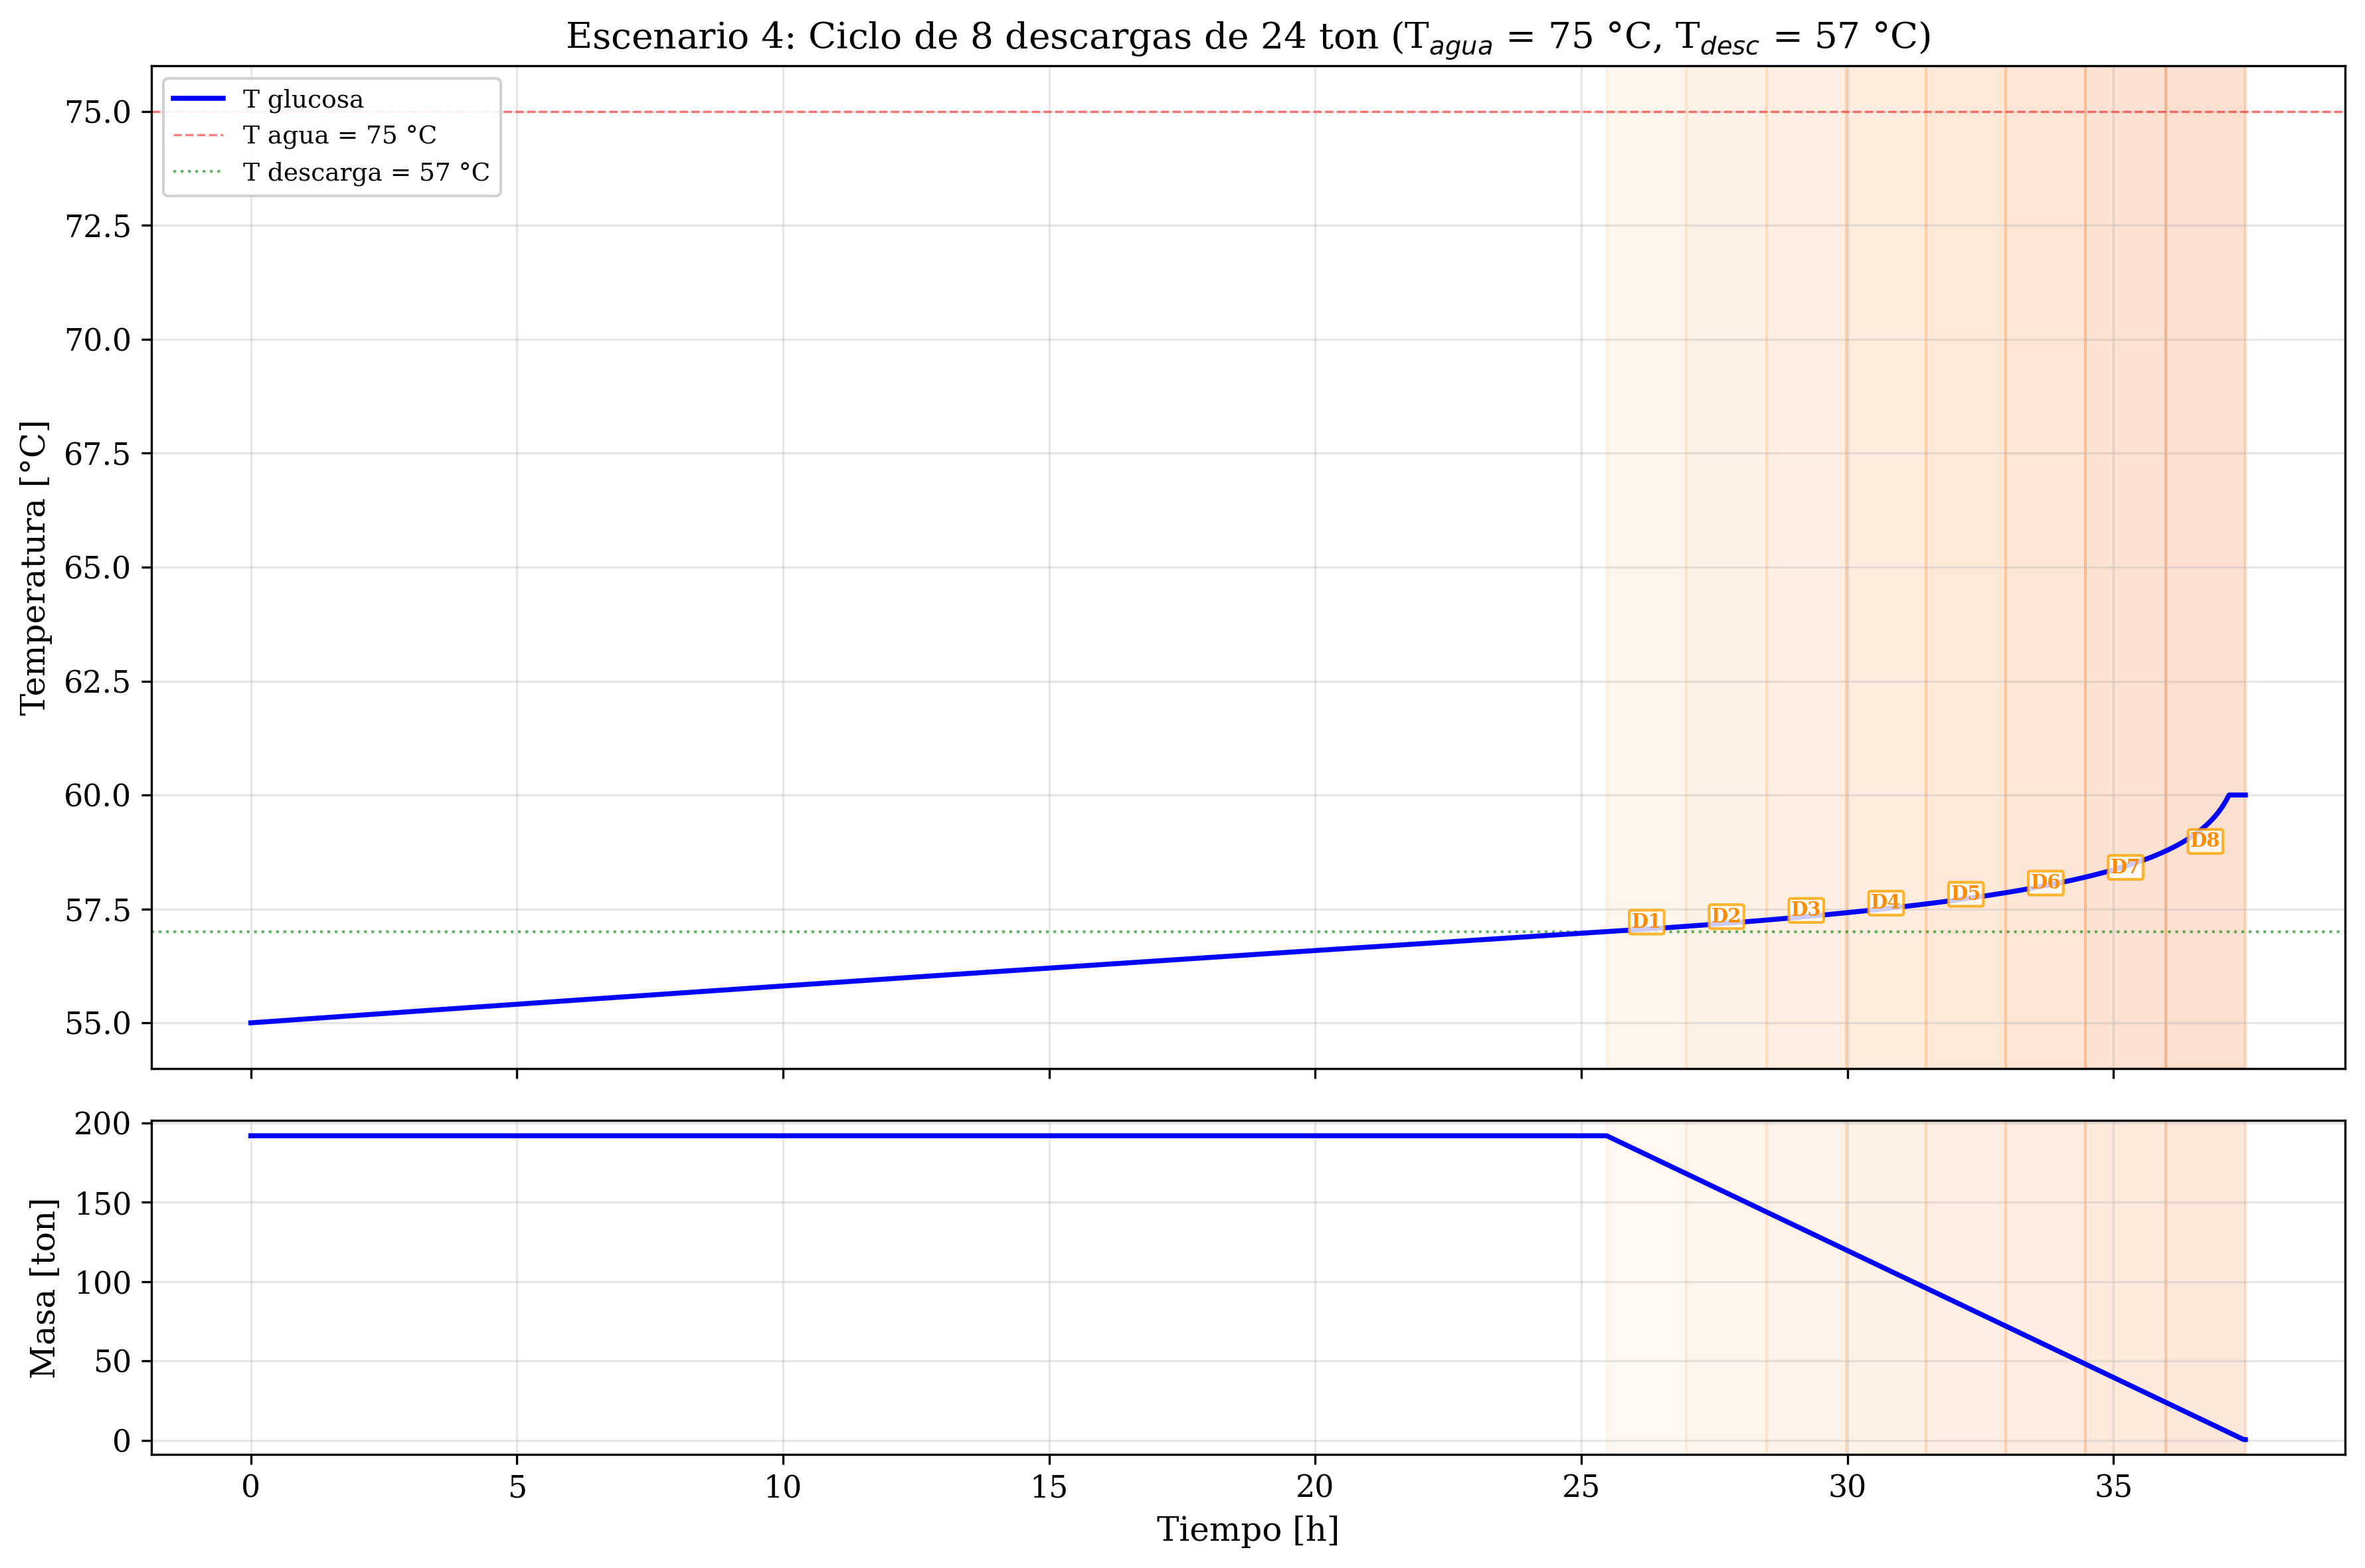
\includegraphics[width=0.85\textwidth]{../figures/escenario4_ciclo_T.png}
	\caption{Dinámica del Ciclo de Despacho (Escenario 4): Evolución de la temperatura (panel superior) y vaciado de masa (panel inferior). Se observa que una vez alcanzado el umbral de 57°C, la temperatura asciende gradualmente favorecida por la reducción de masa.}
	\label{fig:resumen_ciclo_T}
\end{figure}

\begin{figure}[H]
	\centering
	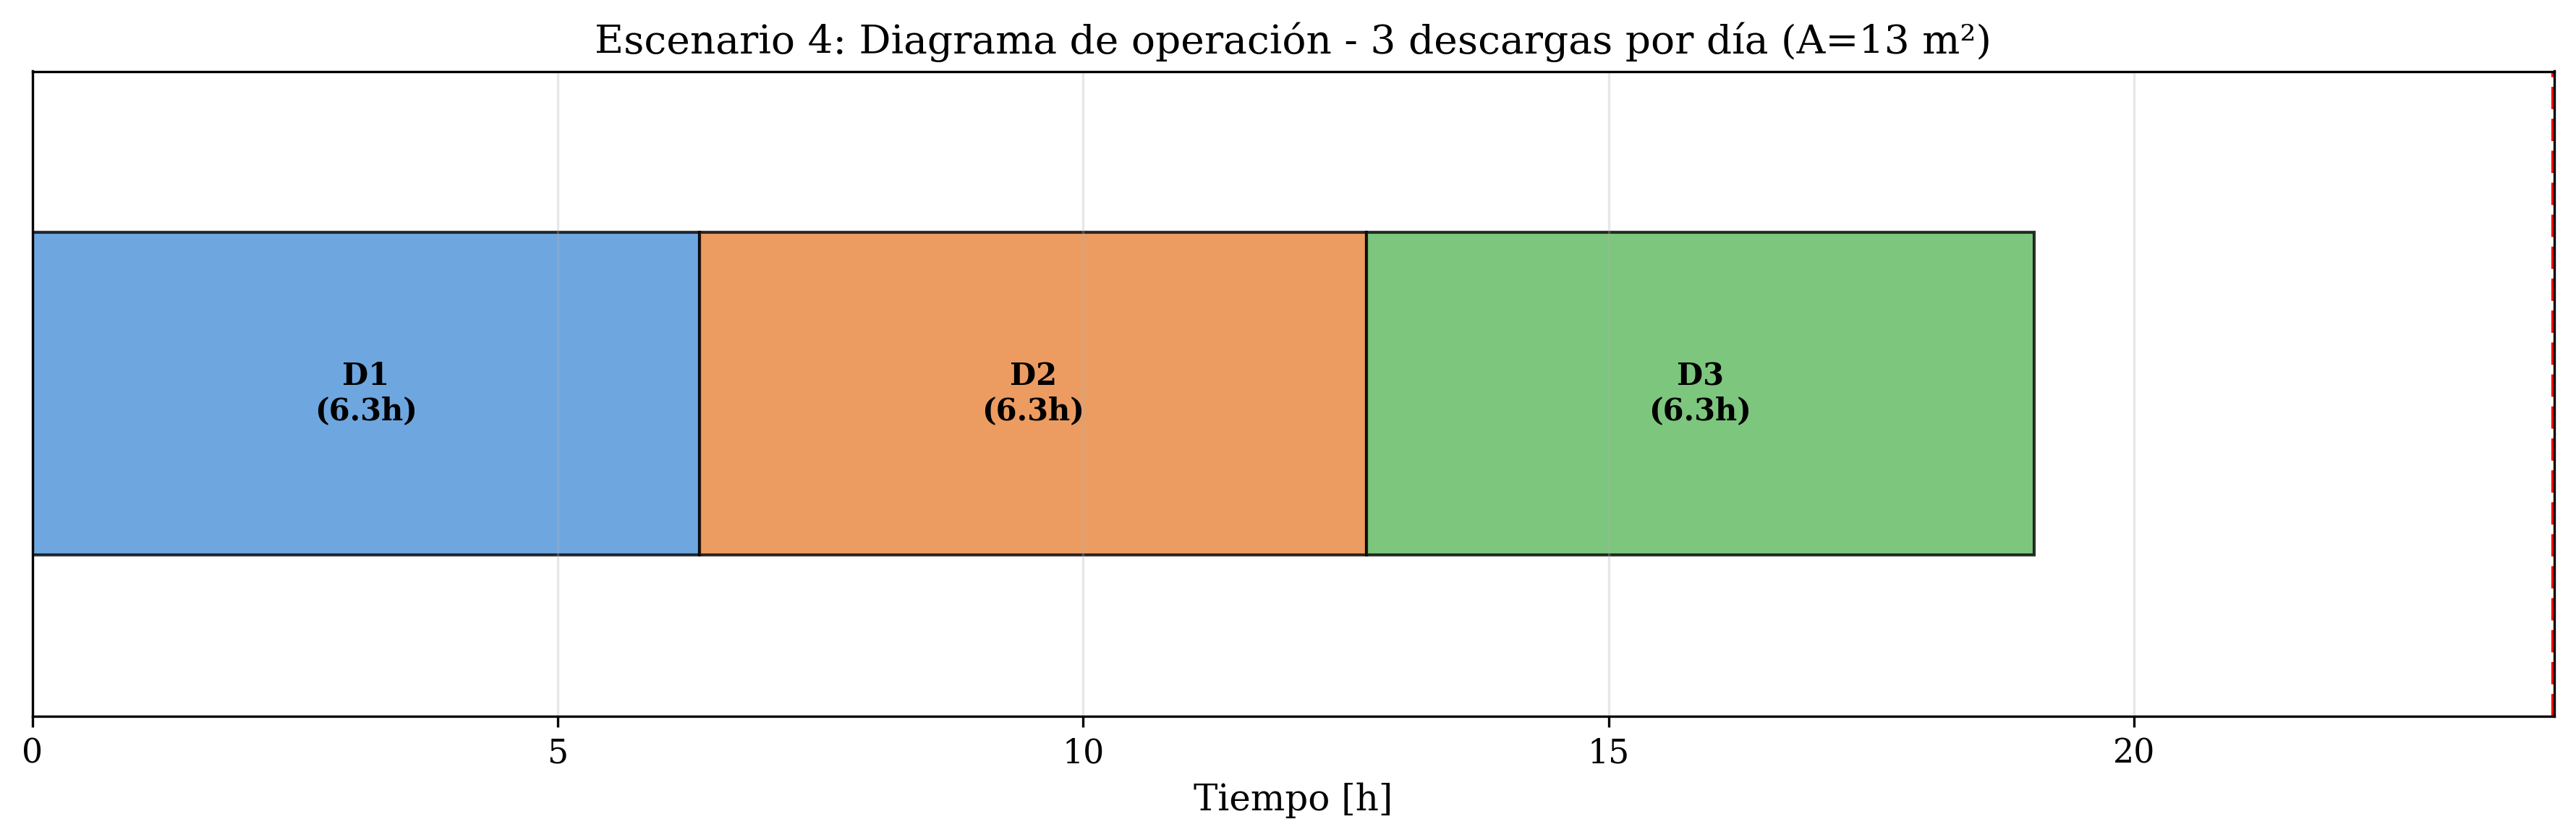
\includegraphics[width=0.85\textwidth]{../figures/escenario4_gantt.png}
	\caption{Cronograma Operativo (Gantt): Distribución temporal del recalentamiento inicial (azul) y las 8 ventanas de carga de 1.5 horas (naranja).}
	\label{fig:resumen_gantt}
\end{figure}

\subsection*{Conclusiones y Recomendaciones Estratégicas}

Las principales deducciones técnicas y directrices de gestión se consolidan en la Tabla~\ref{tab:resumen_conclusiones_recom}, priorizando la integridad del activo y la eficiencia del proceso.

\begin{table}[H]
	\centering
	\caption{Consolidado de conclusiones y recomendaciones técnicas.}
	\label{tab:resumen_conclusiones_recom}
	\setcounter{itemcount}{0}
	\begin{tabularx}{\textwidth}{@{}lX@{}}
		\toprule
		\textbf{Categoría} & \textbf{Conclusión / Recomendación Técnica} \\
		\midrule
		\textbf{Optimización Térmica} & Estandarizar la temperatura del agua de servicio en \textbf{75°C} e instalar \textbf{2'' (50.8 mm) de lana mineral}. Se proyecta una reducción de pérdidas del 91\% y una temperatura superficial segura de 30.8°C. \\
		\midrule
		\textbf{Eficiencia de Proceso} & Implementar una configuración de \textbf{flujo multi-ramal en paralelo} en la chaqueta espiral para optimizar el gradiente térmico y homogeneizar la transferencia de calor en toda la superficie de contacto. \\
		\midrule
		\textbf{Gestión de Integridad} & Se proyecta una vida útil remanente de \textbf{16.3 años} para el cuerpo cilíndrico. Sin embargo, el \textbf{nuevo fondo toriesférico} presenta una vida útil proyectada de \textbf{7.5 años} bajo el criterio del 10\% de margen de diseño, condicionada por el fenómeno de \textbf{corrosión-fatiga} (0.12 mm/año, determinada mediante análisis de espesores en campo) inducido por la operación a 75°C y alta ciclicidad. \\
		\midrule
		\textbf{Refuerzo Estructural} & Ejecutar un plan de refuerzo proactivo en zonas con \textbf{FS < 1.5}. Es imperativa la intervención en el nudillo fondo-cilindro y anclajes (FS $\approx$ 0.71) mediante anillos de rigidización o placas de refuerzo para restaurar los márgenes de ASME VIII Div. 1 y posibilitar la operación al 100\% de llenado. \\
		\bottomrule
	\end{tabularx}
\end{table}

El cumplimiento riguroso de estas directrices garantiza la estabilidad estructural del activo y optimiza la cadena de suministro de glucosa de Ingredion S.A.

\newpage
